\section{Autentikáció és védett útvonalak}

Az alkalmazás autentikációs része email és jelszó alapú bejelentkezésre épül. A belépéshez és regisztrációhoz külön oldalak tartoznak: a \texttt{/login} útvonal a meglévő felhasználók beléptetését, a \texttt{/sign-up} útvonal pedig az új felhasználói fiókok létrehozását kezeli.

A bejelentkezési és regisztrációs űrlapok validációját a \texttt{react-hook-form} végzi. A login form az email címet és a jelszót ellenőrzi, míg a regisztrációs oldal egy megerősítő jelszómezőt is tartalmaz. Sikeres belépés után az alkalmazás a profiloldalra irányítja a felhasználót, hibás adatbevitel vagy sikertelen autentikáció esetén pedig közvetlenül az űrlapon jelenik meg visszajelzés.

\begin{figure}[H]
    \centering
    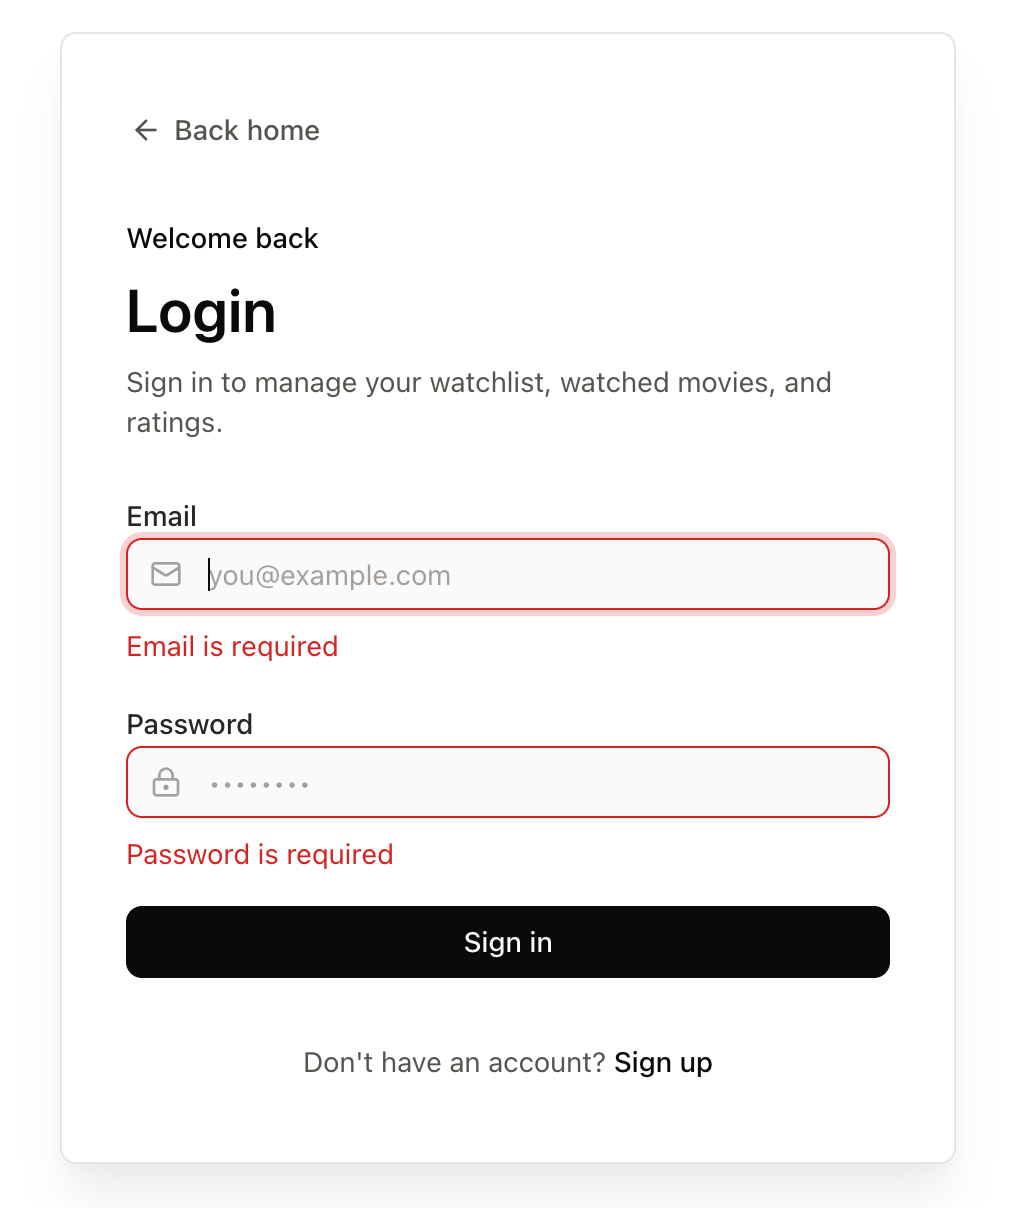
\includegraphics[width=0.52\textwidth]{chapters/chapter-6-implementation/incorrect-login.png}
    \caption{Hibás bejelentkezési kísérlet}
    \label{fig:watchdb-incorrect-login}
\end{figure}

Az autentikációhoz a projekt böngészőoldali és szerveroldali Supabase klienst is használ. A böngészőoldali kliens az űrlapokhoz kapcsolódik, a szerveroldali kliens pedig a védett oldalak és API route-ok esetében kéri le az aktuális felhasználót. A munkamenet cookie-kon keresztül kezelődik, amelynek frissítését a middleware (minden kérés feldolgozása előtt lefutó kód) végzi.

A profiloldal védett útvonalként működik: ha nincs bejelentkezett felhasználó, az alkalmazás a \texttt{/login} oldalra irányítja a látogatót. Aktív session esetén a profiloldal megjeleníti a felhasználóhoz tartozó watched és watchlist listákat.

Ugyanezen az elven működnek az állapotmódosító API route-ok is. A watchlist és watched műveletek előtt a szerveroldali réteg ellenőrzi az aktuális felhasználót, majd az adatbázis műveleteket ehhez a fiókhoz köti.

Ez a felépítés egyértelműen elkülöníti a nyilvános és a személyes funkciókat. A filmkeresés és a film oldalak megtekintése bejelentkezés nélkül is használható, míg a watchlist, a megnézett filmek listája, az értékelés és a profiloldal már felhasználói fiókhoz kötött.
